\documentclass{article}
\usepackage{microtype}
\usepackage{graphicx}
\usepackage{natbib}
\usepackage{amssymb,amsmath,amsthm}
\usepackage{subfigure}
\usepackage{booktabs} % for professional tables
\newtheorem{definition}{Definition}
\newtheorem{theorem}{Theorem}
\DeclareMathOperator*{\argmin}{arg\, min} 
\usepackage{hyperref}
\usepackage{algorithm}
\usepackage{algorithmic}
\usepackage{fullpage}[cm]
\begin{document}

\title{Gradient-based Optimization of the Area Under the Minimum of False Positive and False Negative Functions}
\author{Jonathan Hillman and \\
Toby Dylan Hocking --- toby.hocking@nau.edu}
\maketitle

\begin{abstract}
Receiver Operating Characteristic (ROC) curves are plots of true positive rate versus false positive rate which are useful for evaluating binary classification models, but difficult to use for learning since the Area Under the Curve (AUC) is non-convex.
ROC curves can also be used in other problems that have false positive and true positive rates such as changepoint detection.
We show that in this more general context, the ROC curve is not always monotonic, and so if loops are present the Area Under the Curve (AUC) can be greater than one.
We propose a new differentiable surrogate loss function called the AUM, short for Area Under Min(FP, FN).
We show that the AUM gradient can be efficiently computed and used in a new learning algorithm.
In our empirical study of supervised binary classification and changepoint detection problems, we show that our new AUM minimization algorithm results in improved AUC and comparable speed relative to previous baselines.
\end{abstract}

\section{Introduction}
\label{sec:introduction}
In supervised machine learning problems such as binary classification and changepoint detection, the goal is to learn a function for accurately predicting presence or absence of a class label.
In binary classification there is a prediction for each example; in changepoint detection there is a prediction (change or not) in between each data point in a sequence.
%Our main goal in this research project is to generate a linear model that yields a higher model performance than previously baseline linear models. 
There are numerous ways to analyze a model's performance, but the simplest way is to calculate its accuracy, which is the number or proportion of correctly classified labels.
However using accuracy as the evaluation metric can be problematic for data sets with imbalanced labels or for which the desired weighting of the labels is unknown.
% For example, consider a data set with a high number of positive labels.
% One could generate a model with a high accuracy simply by predicted every label to be positive, without any consideration of the features of the instance.
% This model is essentially useless, as it would never be capable of predicting when an example may have a negative label. 

A popular approach for comparing models in this context is by analyzing their Receiver Operating Characteristic (ROC) curves, which are plots of True Positive Rate (TPR) versus False Positive Rate (FPR).
A single prediction vector for a model can be visualized as a single point in ROC space; the ROC curve is traced by adding a constant real-valued threshold to each prediction in that vector.
Large thresholds result in FPR=TPR=1 and small thresholds result in FPR=TPR=0.
Therefore the Area Under the Curve (AUC) is an evaluation metric which accounts for all possible thresholds or weights for the class labels.
In binary classification, a perfect model has an AUC of 1, a constant model has an AUC of 0.5, and the minimum AUC is 0.


\begin{figure*}[ht]
\vskip 0.2in
\begin{center}
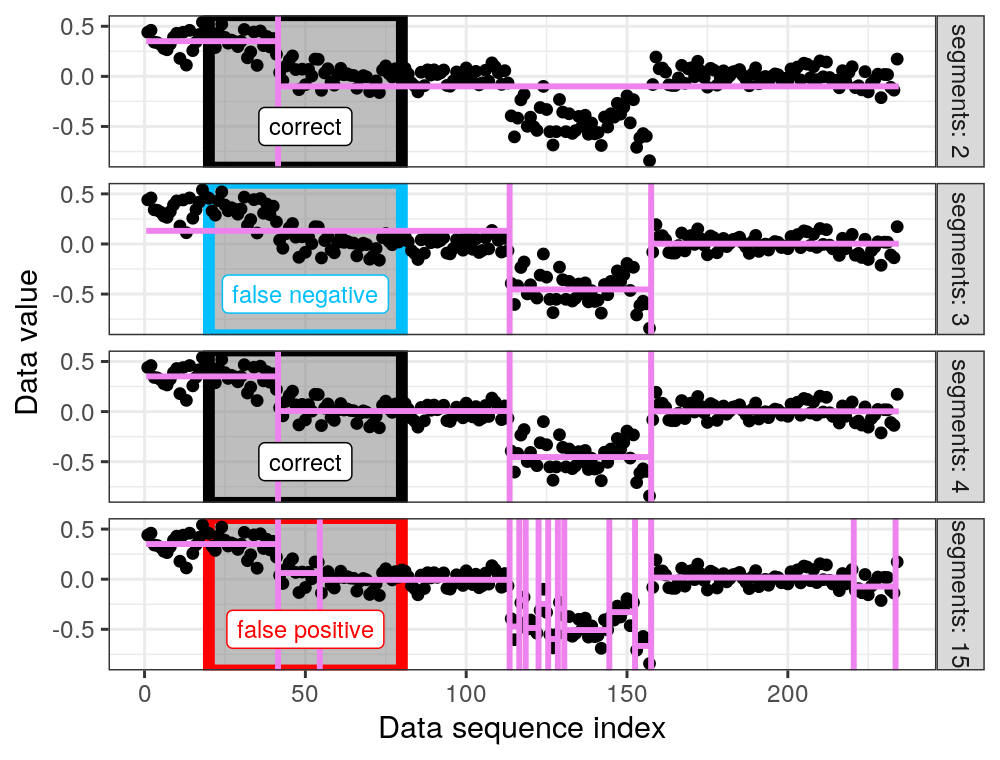
\includegraphics[width=0.55\textwidth]{figure-fn-not-monotonic.png}
%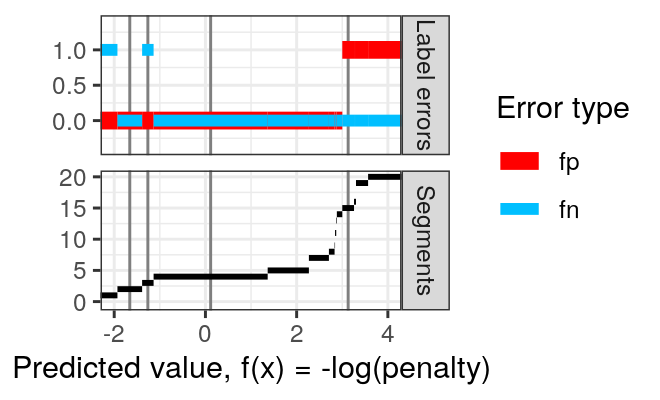
\includegraphics[width=0.45\textwidth]{figure-fn-not-monotonic-error.png}
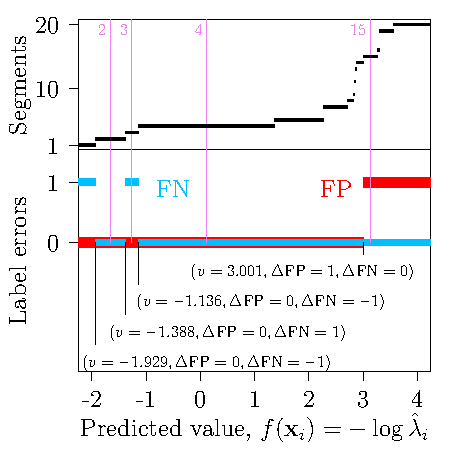
\includegraphics[width=0.44\textwidth]{figure-fn-not-monotonic-error-standAlone.pdf}
\vskip -0.5cm
\caption{Example data for which the ROC curve is non-monotonic. 
\textbf{Left:} a data sequence (black dots) with one label (grey rectangle) in which there should be exactly one predicted changepoint (false negative for no changes when segments=3, false positive for two changes when segments=15).  
\textbf{Right:} selected number of segments (top) and number of label errors (bottom) as a function of predicted values, with vertical violet lines indicating the models shown on the left, and vertical black lines for breakpoints in the error functions. 
%Note how the FN function is not monotonic.
}
\label{fig:fn-not-monotonic}
\end{center}
\vskip -0.2in
\end{figure*}

When AUC is used as the evaluation metric in machine learning, the best algorithm is defined as the one that maximizes test AUC.
In such experiments, we would also like to use the AUC as the objective function for training the model (under the assumption that if the train and test sets are similar, maximizing train AUC should result in maximizing test AUC). 
However, since the AUC is a piecewise constant function of the predicted values, its gradient is zero almost everywhere, and it is therefore impossible to directly optimize using gradient descent algorithms.

In this paper, we study supervised changepoint detection, in which we can compute FPR and TPR as in binary classification.
For binary classification, we can compute a prediction vector which maximizes AUC in the same way as maximizing accuracy --- predict a positive value for each positive label, and a negative value for each negative label.
For changepoint detection, it is also trivial to compute a prediction vector that maximizes accuracy, but it can be non-trivial to compute a prediction vector that maximizes AUC.
%This is because in changepoint detection, the FPR and TPR may be non-monotonic functions of the predicted values, which means that the ROC curve may have loops.
The previous observations motivate this paper, which explores a new loss function and corresponding learning algorithm which we empirically show results in AUC maximization.

\subsection{Contributions}

In Section~\ref{sec:model} we give precise definitions of the AUC and our new AUM loss function, which is the \textbf{A}rea \textbf{U}nder the \textbf{M}inimum of false positive and false negative counts as a function of the prediction threshold.
In Section~\ref{sec:algorithms} we give an efficient algorithm for computing directional derivatives of the AUM with respect to predicted values, which we propose using in gradient descent learning algorithms.
In Section~\ref{sec:results} we provide an empirical study of supervised changepoint detection problems, and show that minimizing the AUM corresponds to maximizing the AUC (with respect to train and test sets).

\subsection{Related work}
\label{sec:related-work}

%TODO Jon citations

Related work on AUC optimization for binary classification falls into two categories: gradient
learning algorithms based on re-weighting or approximation, and
discrete learning algorithms such as decision trees.
\citet{ferri2002learning, cortes2004auc} proposed expressions for the expected value
and the variance of the AUC for a fixed error rate, in an attempt to maximize the AUC with different nonlinear algorithms.
\citet{wang2015optimizing} incorporated unlabeled data to make an unsupervised AUC maximization algorithm.
\citet{yan2003optimizing} proposed a global approximation of AUC which was then used in several other algorithms.
For example, \citet{castro2008optimization} used that approxmation to propose the AUCtron algorithm which learns a linear model.
Other algorithms have been proposed to obtain approximations of the global AUC value \citep{ rakotomamonjy2004optimizing, herschtal2004optimising, herschtal2006area, calders2007efficient}.
\citet{joachims2005multivariate} proposed a quadratic time support vector machine algorithm for AUC maximization based on a pairwise loss function.
\citet{Han2010} proposed an active learning algorithm for computing a linear model that maximizes the AUC.
\citet{zhao2011online} implemented an online learning algorithm that maximizes the AUC.
\citet{yuan2020auc} proposed a new surrogate objective function (AUC margin loss) and \citet{yuan2021federated} proposed a federated learning algorithm.

In supervised changepoint detection, learning is often limited to grid search \citep{Hocking2013bioinformatics, Hocking2017bioinfo, Liehrmann2021chipseq}. 
More sophisticated learning algorithms use linear models and non-linear decision trees that minimize convex surrogates of the label error \citep{Hocking2013icml, Hocking2014,  Hocking2015, Drouin2017, Hocking2020psb}.
ROC curves and AUC are used to evaluate prediction accuracy of learned penalty functions \citep{Maidstone2016, Hocking2020jmlr}.


% \begin{figure*}[ht]
% \vskip 0.2in
% \begin{center}
% 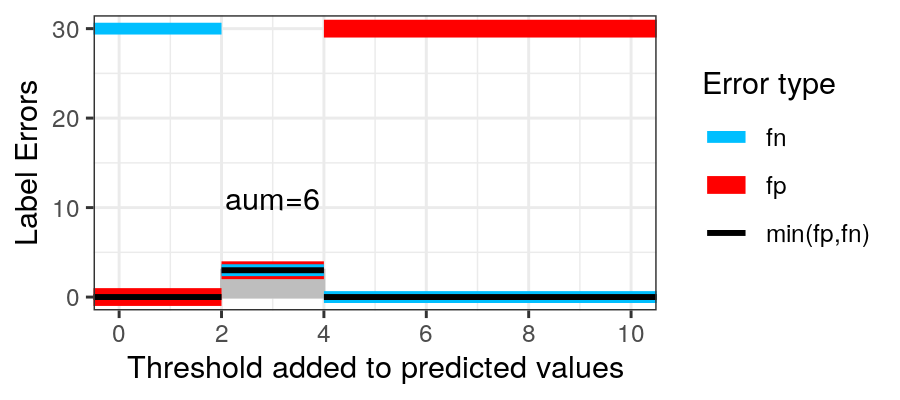
\includegraphics[height=2in]{figure-more-than-one-less-aum.png}
% 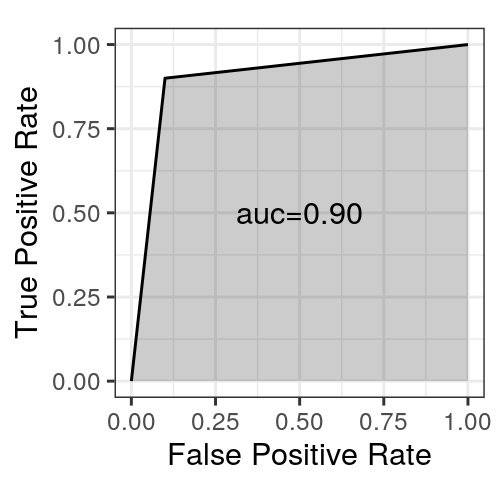
\includegraphics[height=2in]{figure-more-than-one-less-auc.png}
% \vskip -0.5cm
% \caption{Synthetic example typical of binary classification, with monotonic FP/FN functions (left) that result in a monotonic ROC curve (right).
% The q values are indices in the sequence of points on the ROC curve (and corresponding intervals of the FP/FN functions).
% \textbf{Left:} the AUM (grey area) is defined as the area under the minimum of FP and FN functions.
% \textbf{Right:} the AUC is more than 1 due to the loop which results in double counting the dark grey area (but single counting the red area which is positive counted twice and negative counted once).
% }
% \label{fig:less}
% \end{center}
% \vskip -0.2in
% \end{figure*}




\begin{figure*}[t!]
\vskip 0.2in
\begin{center}
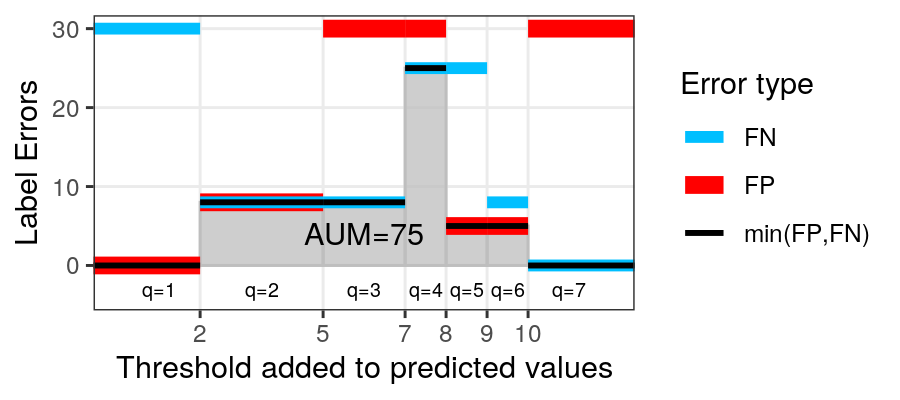
\includegraphics[height=1.8in]{figure-more-than-one-more-aum.png}
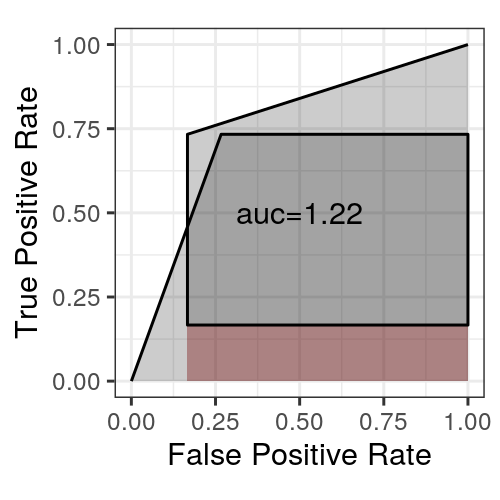
\includegraphics[height=1.8in]{figure-more-than-one-more-auc.png}
\vskip -0.5cm
\caption{Synthetic example showing how non-monotonic FP/FN functions (left) can result in a looping ROC curve (right).
The q values are indices in the sequence of points on the ROC curve (and corresponding intervals of the FP/FN functions).
\textbf{Left:} the AUM (grey area) is defined as the area under the minimum of FP and FN functions.
\textbf{Right:} the AUC is more than 1 due to the loop which results in double counting the dark grey area (but single counting the red area which is positive counted twice and negative counted once).
}
\label{fig:more}
\end{center}
\vskip -0.2in
\end{figure*}



\section{Models and Definitions}
\label{sec:model}
We begin by reviewing supervised binary classification and changepoint detection, then give definitions for AUC and the new AUM loss function.
\subsection{Review of supervised binary classification}

In supervised binary classification we are given a set of $n$ labeled training examples, $\{(\mathbf x_i, y_i)\}_{i=1}^n$ where $\mathbf x_i\in\mathbb R^p$ is an input feature vector for one observation and $y_i\in\{-1,1\}$ is a binary output/label.
The goal of binary classification is to learn a function $f:\mathbb R^p\rightarrow \mathbb R$ which outputs a real-valued prediction with the same sign as the corresponding label.
Learning algorithms such as logistic regression and support vector machines involve minimizing a convex loss function $\ell:\mathbb R\times \{-1,1\}$, summed over all training examples:
\begin{equation}
\label{eq:loss-sum-over-examples}
    \mathcal L(f) =  \sum_{i=1}^n \ell[ f(\mathbf x_i), y_i].
\end{equation}
After a function $f$ has been learned using the training data, it can be evaluated by computing non-convex evaluation metrics such as the zero-one loss or the AUC with respect to a held-out test set.

\subsection{Review of supervised changepoint detection}

In supervised changepoint detection \citep{Hocking2013icml}, we have  $n$ labeled training examples. 
Each labeled training example $i\in\{1,\dots,n\}$ has a corresponding data sequence vector $\mathbf z_i$ and label set $L_i$.
For example in Figure~\ref{fig:fn-not-monotonic} we show a data sequence $\mathbf z_i$ with a label set $L_i$ that contains one positive label (grey region in which there should be exactly one predicted changepoint).
Dynamic programming algorithms can be used on the data sequence $\mathbf z_i$ to compute a path of optimal changepoint models $\mathbf {\hat m}^k_i$ for different model sizes $k\in\{1,2,\dots\}$  \citep{Maidstone2016}.
For example in Figure~\ref{fig:fn-not-monotonic} (left) we show four models in the path (with $k=2,3,4,15$ segments).
The label set $L_i$ can be used to compute the number of false positive and false negative labels with respect to any predicted set of changepoints (false positives for too many changepoints, false negatives for not enough changepoints).
Each example $i$ also has a model selection function $k^*_i:\mathbb R^+_0 \rightarrow \{1,2,\dots\}$ which maps a non-negative penalty value $\hat \lambda_i$ to a selected model size $k^*_i(\hat \lambda_i)$ (Figure~\ref{fig:fn-not-monotonic}, right bottom).
We assume there is a fixed feature map $\phi$ which can be used to compute a feature vector $\mathbf x_i = \phi(\mathbf z_i)\in\mathbb R^p$ for each labeled example.

We want to learn a function $f:\mathbb R^p\rightarrow \mathbb R$ which inputs a feature vector and outputs a real-valued prediction that is used as a negative log penalty value, $f(\mathbf x_i) = -\log \hat \lambda_i$.
The goal is to predict model sizes $k^*_i(\hat \lambda_i)$ that result in minimal label errors. 
Since the label error function is non-convex like the zero-one loss in binary classification (Figure~\ref{fig:fn-not-monotonic}, right top), previous learning algorithms instead use the gradient with respect to a convex surrogate such as a hinge loss \citep{Hocking2013icml,Drouin2017} or a censored regression loss \citep{barnwal2021aftxgboost}.

\subsection{Definition of false positive and negative functions}
\label{sec:def-fp-fn}
%Now we assume that $n$ is the number of related problems for which we want to make a real-valued prediction (same as the number of labeled training examples in binary classification).
%For each problem $i \in \{1, 2, \dots n\}$, we make a real-valued prediction $f(\mathbf x_i) = \hat y_i\in\mathbb R$, and let $\mathbf{ \hat y}$ be the $n$-dimensional vector with $\hat y_i$ in each coordinate $i\in\{1,\dots,n\}$.

In this paper, we assume the following general learning context in which supervised binary classification and changepoint detection are specific examples. 
For each labeled training example $i$, we have one or more labels such that there are at most $\text{FNP}_i\in\mathbb Z_+=\{0, 1, \dots\}$  false negatives possible and $\text{FPP}_i\in\mathbb Z_+$ false positives possible.
Given a real-valued prediction $\hat y_i=f(\mathbf x_i)\in\mathbb R$, we can use the labels to compute the number of predicted false positives $\text{FP}_i(\hat y_i)\in \{0, \dots, \text{FPP}_i\}$ and false negatives $\text{FN}_i(\hat y_i)\in\{0, \dots, \text{FNP}_i\}$.
The $\text{FP}_i,\text{FN}_i$ functions return the number of false positive and false negative labels for a given predicted value $\hat y_i$. 

\paragraph{Exact representation using breakpoints.} 
By convention we assume that the $\text{FP}_i,\text{FN}_i$ functions are right continuous; 
that the $\text{FP}_i$ functions start at zero, $\lim_{x\rightarrow -\infty}\text{FP}_i(x)=0$; 
and the $\text{FN}_i$ functions end at zero, $\lim_{x\rightarrow \infty} \text{FN}_i(x)=0$. 
These assumptions ensure that (1) our proposed AUM loss function will always be finite, and (2) it can be computed efficiently by representing the error functions exactly using a finite set of breakpoints $(v,\Delta\text{FP},\Delta\text{FN})$. 
Each $v\in\mathbb R$ is a predicted value where there are changes $\Delta\text{FP},\Delta\text{FN}$ in the error functions, $\text{FP}_i(v)-\lim_{x\rightarrow v^-} \text{FP}_i(x)= \Delta\text{FP}$ and similar for FN.
For example, in Figure~\ref{fig:fn-not-monotonic} the error functions can be exactly represented by a set of four such breakpoints.
These breakpoints will be used when computing our proposed loss function and learning algorithm. 


\paragraph{Case of binary classification.} 
In the case of binary classification, for all positive examples $i:y_i=1$ we have 
 $\text{FPP}_i=0$, 
 $\text{FNP}_i=1$,
 $\text{FP}_i(\hat y) = 0$,
 $\text{FN}_i(\hat y) = I(\hat y < 0)$,
% \begin{eqnarray}
%   \text{FPP}_i&=&0,\\
%   \text{FNP}_i&=&1, \\
%   \text{FP}_i(\hat y) &=& 0, \\
%   \text{FN}_i(\hat y) &=& I(\hat y < 0),
% \end{eqnarray}
where $I$ is the indicator function (outputs 1 if argument is true, 0 otherwise).
For all negative examples $i:y_i=-1$,
  $\text{FPP}_i=1$,
  $\text{FNP}_i=0$,
  $\text{FP}_i(\hat y) = I(\hat y \geq 0)$, 
  $\text{FN}_i(\hat y) = 0$.
% \begin{eqnarray}
%   \text{FPP}_i&=&1,\\
%   \text{FNP}_i&=&0, \\
%   \text{FP}_i(\hat y) &=& I(\hat y \geq 0), \\
%   \text{FN}_i(\hat y) &=& 0.
% \end{eqnarray}
Note that $\text{FP}_i$ is either constant/zero (for positive examples) or non-decreasing (for negative examples), and $\text{FN}_i$ is either constant/zero (for negative examples) or non-increasing (for positive examples).
These functions can be exactly represented by the breakpoint
$(v=0,\Delta\text{FP}=0,\Delta\text{FN}=-1)$ for all positive examples, and 
$(v=0,\Delta\text{FP}=1,\Delta\text{FN}=0)$ for all negative examples.

\paragraph{Case of changepoint detection.} 
In changepoint detection, we have more general $\text{FP}_i$ and $\text{FN}_i$ functions that can be non-monotonic.
For example, in Figure~\ref{fig:fn-not-monotonic}, we show a data sequence with one positive label (in which there should be exactly one predicted changepoint).
Predicting no changepoint in this label results in a false negative, and predicting two changepoints in this label results in a false positive. 
Therefore, we have $\text{FPP}_i=\text{FNP}_i=1$ for this particular example $i$;
% > err.list$model.errors[, .(min.log.lambda, max.log.lambda, segments, fp, fn)]
%     min.log.lambda max.log.lambda segments fp fn
%  1:           -Inf      -3.566634       20  1  0
%  2:      -3.566634      -3.301154       19  1  0
%  3:      -3.301154      -3.258186       16  1  0
%  4:      -3.258186      -3.000918       15  1  0
%  5:      -3.000918      -2.881569       14  0  0
%  6:      -2.881569      -2.868007       13  0  0
%  7:      -2.868007      -2.842141       11  0  0
%  8:      -2.842141      -2.831636        9  0  0
%  9:      -2.831636      -2.707501        8  0  0
% 10:      -2.707501      -2.268619        7  0  0
% 11:      -2.268619      -1.365036        5  0  0
% 12:      -1.365036       1.136433        4  0  0
% 13:       1.136433       1.388073        3  0  1
% 14:       1.388073       1.929300        2  0  0
% 15:       1.929300            Inf        1  0  1
the false positive function is non-decreasing, $\text{FP}_i(\hat y_i) \approx I(\hat y_i \geq 3.001)$, and the false negative function is not monotonic, $\text{FN}_i(\hat y_i) \approx I[\hat y_i \in (\infty, -1.929)\cup (-1.388, -1.136)]$.
When the false negative function is non-monotonic, the true positive rate is also non-monotonic (the ROC curve can move down as well as up when prediction threshold is increased).
Given a pre-computed path of changepoint models with loss/size values, the exact breakpoints $(v,\Delta\text{FP},\Delta\text{FN})$ in such error functions can be efficiently computed using a linear time algorithm \citep{Vargovich2020arxiv}.

\begin{figure*}[t]
\vskip 0.2in
\begin{center}
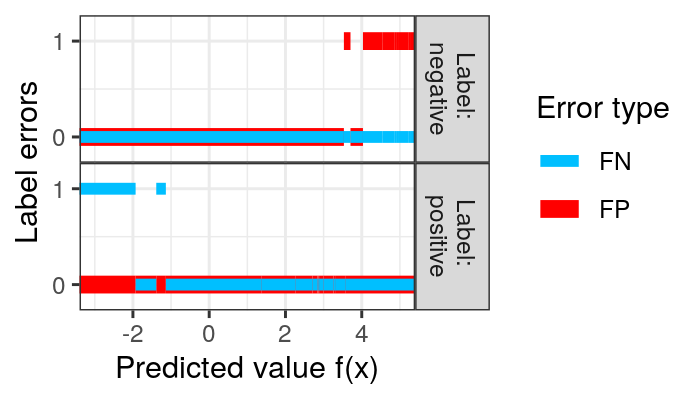
\includegraphics[height=3.7cm]{figure-aum-convexity-profiles.png}
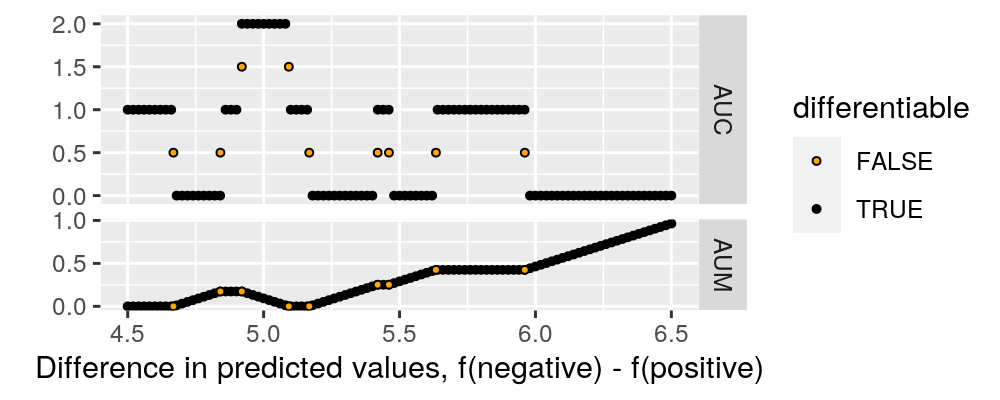
\includegraphics[height=3.7cm]{figure-aum-convexity.png}
\vskip -0.5cm
\caption{Real data example showing that it is possible to have AUC greater than one.
\textbf{Left:} error functions for two labeled examples in a real changepoint detection data set.
\textbf{Right:} AUM and AUC values as a function of the difference in predicted values between the two labeled examples.
When the difference is around 5, we have AUC=2.
We can see that the AUC is a piecewise constant function of the predicted values, whereas the AUM is a continuous piecewise linear function.
It can be seen in this example that at differentiable points, AUM=0 implies AUC=1 (but the converse is false).
}
\label{fig:aum-convexity}
\end{center}
\vskip -0.2in
\end{figure*}

\subsection{Definition of ROC curve and AUC}

In this section, we show how the previously defined functions can be used to define the ROC curve and the AUC.
Given a vector of predictions $\mathbf{\hat y}$, we define the False Positive Total (FPT) and False Negative Total (FNT) as
\begin{eqnarray}
 \text{FPT}(\mathbf {\hat y}) &=&
 \sum_{i=1}^n \text{FP}_i(\hat y_i), \\
 \text{FNT}(\mathbf {\hat y}) &=&
 \sum_{i=1}^n \text{FN}_i(\hat y_i).
\end{eqnarray}
For a prediction threshold $t\in\mathbb R$, the False Positive Rate (FPR) and True Positive Rate (TPR) functions are
\begin{eqnarray}
 \text{FPR}_{\mathbf {\hat y}}(t) &=&
 \frac{1}{\sum_{i=1}^n \text{FPP}_i } 
 \text{FPT}(\mathbf {\hat y}+t), \\
 \text{TPR}_{\mathbf {\hat y}}(t) &=&
 1 - 
 \frac{1}{\sum_{i=1}^n \text{FNP}_i } 
 \text{FNT}(\mathbf {\hat y}+t).
%  \text{FNR}_{\mathbf {\hat y}}(t) &=&
%  \frac{1}{\sum_i \text{FNP}_i } 
%  \text{FNT}(\mathbf {\hat y}+t),\\
%  \text{TPR}_{\mathbf {\hat y}}(t) &=&
%  1 - \text{FNR}_{\mathbf {\hat y}}(t)
\end{eqnarray}
The ROC curve for a given prediction vector $\mathbf {\hat y}$ is the plot of $\text{TPR}_{\mathbf {\hat y}}(t) $ versus $\text{FPR}_{\mathbf {\hat y}}(t) $ as the prediction threshold $t$ is varied from $-\infty$ to $\infty$.
The AUC is the integral,
\begin{equation}
    \text{AUC}(\mathbf{\hat y}) = 
    \int \text{TPR}_{\mathbf {\hat y}}(t) 
    d\, \text{FPR}_{\mathbf{\hat y}}(t).
\end{equation}
Assuming the $\text{FPT}$ and $\text{FNT}$ functions are piecewise constant (as in binary classification and changepoint detection) then the ROC curve can be described as a sequence of $Q$ points 
$\{(\text{fpr}
(\mathbf {\hat y})
_q, \text{tpr}
(\mathbf {\hat y})
_q)\}_{q=1}^Q$ in ROC space (note that this sequence of points depends on the predicted values $\mathbf {\hat y}$).
The first point $q=1$ corresponds to prediction threshold $t=-\infty$ which results in TPR=0 and FPR=0; the last point $q=Q$ is for $t=\infty$ which results in TPR=1 and FPR=1 (Figure~\ref{fig:more}).
The AUC can be computed using this sequence,
\begin{eqnarray}
\label{eq:auc-seq}
&&\text{AUC}(\mathbf {\hat y}) = \\
  &&  \sum_{q=1}^{Q-1} 
    (\text{fpr}
    (\mathbf {\hat y})
    _{q+1} - \text{fpr}
    (\mathbf {\hat y})
    _q)
    (\text{tpr}
    (\mathbf {\hat y})
    _{q} + \text{tpr}
    (\mathbf {\hat y})
    _{q+1})/2.\nonumber
\end{eqnarray}
In binary classification we have $\text{fpr}(\mathbf {\hat y})_{q} \leq \text{fpr}(\mathbf {\hat y})_{q+1}$ which means while tracing the ROC curve there are no moves to the left, and all the terms in the sum above are positive.
In fact this is also true of changepoint detection problems for which all the $\text{FP}_i$ functions are non-decreasing. 
In these cases the ROC curve is monotonic, with $\text{AUC}(\mathbf {\hat y})\in[0,1]$ for any predicted values $\mathbf {\hat y}$.

\subsection{Existence of non-monotonic ROC curves}

However if some of the $\text{FP}_i$ functions are not monotonic, then it is possible to have $\text{fpr}(\mathbf {\hat y})_{q} > \text{fpr}(\mathbf {\hat y})_{q+1}$ which results in negative terms in the AUC equation~(\ref{eq:auc-seq}). 
Furthermore if some of the $\text{FN}_i$ functions are not monotonic, then the ROC curve can contain loops which double count some area in ROC space.
For a simple synthetic example, consider the FP/FN functions and corresponding ROC curves in Figure~\ref{fig:more}.
In this example, the ROC curve has area greater than one because it contains a loop which double-counts a large portion of ROC space.
%This begs the question, is it desirable to maximize the AUC? If so then how can it be maximized efficiently? If not then should we optimize some other criterion?
% In typical binary classification problems it is desirable to maximize the AUC because the ROC curve is monotonic, which means that most points on the curve represent an optimal tradeoff between true positive and false positive rates.
% However in this more general context it is no longer true that most points on the ROC curve result in an optimal tradeoff --- when there are loops there are thresholds which are highly sub-optimal in terms of TPR and/or FPR.

But does this happen in real data? Yes, in real changepoint detection problems such as Figure~\ref{fig:fn-not-monotonic} it is clearly possible to have error functions which are non-monotonic.
Furthermore, in Figure~\ref{fig:aum-convexity} (left) we show error curves for two labeled examples from another real changepoint detection data set.
One example has a positive label that results in a non-monotonic false negative function, and the other example has a negative label that results in a non-monotonic false positive function.
% In general with non-monotonic false positive and false negative functions, it is not tractable to compute predictions which result in max AUC.
% Since there are only two labeled examples in this case, we can explore the relationship between AUC and AUM via a grid search over the difference in predicted values.
When the predicted value for the negative example is about 5 greater than the predicted value for the positive example, we observe AUC=2 (Figure~\ref{fig:aum-convexity}, right).
This is the result of a loop in ROC space, indicating that there is some prediction threshold that results in (FPR=1,TPR=0) which corresponds to 100\% error and 0\% accuracy.
Therefore, maximizing the AUC may not be a good optimization objective; instead, we would like a monotonic ROC curve with AUC=1 that avoids thresholds with such large error rates.
We therefore propose a new surrogate loss function for this objective in the next section.

\subsection{Proposed loss function: AUM}

In this section we propose the AUM loss function, which is short for Area Under Min(FP,FN).
The intuition behind the AUM is that we want to minimize the number of prediction thresholds that result in large error rates.
To formally define the AUM we must first define the minimum of total false positives and false negatives, 
\begin{equation}
    M(\mathbf {\hat y}) = 
    \min\{
    \text{FPT}(\mathbf{\hat y}),
    \text{FNT}(\mathbf{\hat y})
    \}.
\end{equation}
Then we define the AUM as 
\begin{equation}
\label{eq:AUM}
    \text{AUM}(\mathbf {\hat y}) =
    \int_{-\infty}^{\infty}
    M(\mathbf {\hat y} + t)\, dt.
\end{equation}
In summary, we compute AUM by integrating the $M$ function over all possible prediction thresholds $t$.
Geometrically, this corresponds to the area under the minimum of total false positive and false negative functions (Figure~\ref{fig:more}, left).
%Since $M$ is the minimum of the total false positives and false negatives over all examples,
A few interesting properties should be immediately apparent.
\begin{description}
    \item[Finite.] 
Since $\text{FP}_i(-\infty)=0$ and $\text{FN}_i(\infty)=0$ for all $i$ (by assumption), we have $M(\mathbf{\hat y}\pm\infty)=0$, which means 
% the minimum is zero at both extreme prediction thresholds. 
% Therefore 
the AUM integral~(\ref{eq:AUM}) is finite, $\text{AUM}(\mathbf{\hat y})<\infty$.
\item[Non-negative.] Since the label error is never negative, the AUM integral is never negative, $\text{AUM}(\mathbf{\hat y})\geq 0$.
% \item[Zero condition.] We have $\text{AUM}(\mathbf{\hat y})=0$ if and only if $M(\mathbf{\hat y}+t)=0$ for all thresholds $t$.
\item[Convexity.] If all of the $\text{FP}_i$ and $\text{FN}_i$ functions are monotonic, then the AUM is convex.
\item[Other properties.] The AUM is continuous, piecewise linear, and differentiable almost everywhere. 
\end{description}
%Exploring the precise relationship between AUM and AUC is an interesting direction for future theoretical work.
We observed empirically that non-differentiable points in the AUM coincide with discontinuities in AUC (Figure~\ref{fig:aum-convexity}, right).
Furthermore we observed that at differentiable points, 
if $\text{AUM}(\mathbf{\hat y})=0$ then
$\text{AUC}(\mathbf{\hat y})=1$; 
the converse is clearly false, however (Figure~\ref{fig:aum-convexity}, right).
In this figure it can also be seen that for all predictions with maximal AUC=2, we have $\text{AUM}>0$, which means there are some prediction thresholds which result in FP=FN=1.
This observation suggests that instead of maximizing AUC, it may be preferable to minimize AUM as a surrogate loss, to obtain AUC=1. 
We therefore propose an AUM gradient descent learning algorithm in the next section.

\section{Algorithms}
\label{sec:algorithms}

In this section we propose algorithms for computing the AUM and its gradient, and for learning a linear model.

\subsection{Overview of AUM computation}
\label{sec:algo-aum-overview}
%   aum <- fp.fn.totals[, sum(ifelse(
%     min.fp.fn==0, 0, min.fp.fn*(max.thresh-min.thresh)))]
Computing the AUM is similar to the AUC, in that we must compute error/accuracy rates for each possible prediction threshold. 
First let $\{(
\text{fpt}
(\mathbf {\hat y})
_q, \text{fnt}
(\mathbf {\hat y})
_q,
 \tau
(\mathbf {\hat y})
_q
)\}_{q=1}^Q$ 
be a sequence of $Q$ tuples, each of which corresponds to a point on the ROC curve (Figure~\ref{fig:more}).
The fpt/fnt are false positive/negative totals whereas $\tau$ are prediction threshold values 
% which we assume are increasing, $\tau
% (\mathbf {\hat y})
% _q < \tau
% (\mathbf {\hat y})
% _{q+1}$.
which we assume are increasing, $ -\infty = \tau
(\mathbf {\hat y})
_0 < \cdots <  \tau
(\mathbf {\hat y})
_Q = \infty$.
For each $q\in\{1,\dots,Q\}$ we have 
$\text{FPT}(\mathbf{\hat y}+t)=\text{fpt}(\mathbf {\hat y})_q$
and
$\text{FNT}(\mathbf{\hat y}+t)=\text{fnt}(\mathbf {\hat y})_q$
for all $t\in(\tau(\mathbf {\hat y})_{q-1}, \tau(\mathbf {\hat y})_q)$.
Then we define $m(\mathbf {\hat y})_q = \min\{
    \text{fpt}(\mathbf {\hat y})_q , \, 
    \text{fnt}(\mathbf {\hat y})_q
\}$ and so since 
$m(\mathbf {\hat y})_1=m(\mathbf {\hat y})_Q=0$ the AUM can be computed via
\begin{equation}
\label{eq:AUM-computation}
    \text{AUM}(\mathbf {\hat y}) =
    \sum_{q=2}^{Q-1}
    [ \tau(\mathbf {\hat y})_{q} - \tau(\mathbf {\hat y})_{q-1} ]
    m(\mathbf {\hat y})_q.
\end{equation}
For example, in Figure~\ref{fig:more} there are $Q=7$ tuples (points on the ROC curve), five of which result in a positive AUM value; total AUM is 75.

\subsection{Details of AUM computation}
\label{sec:algo-aum-details}

In previous sections we have assumed that a sequence of $Q$ points on the ROC curve (or equivalently intervals of FP/FN functions) can be computed, and in this section we explain how to do that.
Recall from Section~\ref{sec:def-fp-fn} that the $\text{FP}_i,\text{FN}_i$ functions have an exact representation in terms of breakpoints.
Let there be a total of $B$ breakpoints in the error functions for all $n$ observations, where each breakpoint $b\in\{1,\dots, B\}$ is represented by the tuple $(v_b, \Delta\text{FP}_b, \Delta\text{FN}_b, \mathcal I_b)$.
The $\mathcal I_b\in\{1,\dots,n\}$ is an observation index, so there are changes $\Delta\text{FP}_b, \Delta\text{FN}_b$ at predicted value $v_b\in\mathbb R$ in the error functions $\text{FP}_{\mathcal I_b},\text{FN}_{\mathcal I_b}$ (Figure~\ref{fig:fn-not-monotonic}). 

Given a prediction vector $\mathbf{\hat y}\in\mathbb R^n$ we can compute a prediction threshold $t_b= v_b - \hat y_{\mathcal I_b}$ for each breakpoint $b\in\{1,\dots,B\}$, along with error values
\begin{eqnarray}
  \underline{\text{FP}}_b &=& \sum_{j: t_j \leq t_b} \Delta\text{FP}_j, \\
  \overline{\text{FP}}_b &=& \sum_{j: t_j < t_b} \Delta\text{FP}_j, \\
  \underline{\text{FN}}_b &=& \sum_{j: t_j \geq t_b} - \Delta\text{FN}_j, \\
  \overline{\text{FN}}_b &=& \sum_{j: t_j > t_b} - \Delta\text{FN}_j.
\end{eqnarray}
The $\underline{\text{FP}}_b, \underline{\text{FN}}_b$ are the error values before the threshold $t_b$, whereas $\overline{\text{FP}}_b, \overline{\text{FN}}_b$ are the error values after the threshold. 

We sort the breakpoints by threshold, which is a log-linear $O(B\log B)$ time operation.
This yields a permutation $\{s_1,\dots, s_B\}$ of the indices $\{1,\dots,B\}$ such that for every $q\in\{2,\dots,B\}$ we have $t_{s_{q-1}} \leq  t_{s_q}$.
All of the error values $\underline{\text{FP}}_b,\overline{\text{FP}}_b,\underline{\text{FN}}_b,\overline{\text{FN}}_b$, for every $b\in\{1,\dots,B\}$, can then be computed in linear $O(B)$ time.
In terms of the notation of Section~\ref{sec:algo-aum-overview}, we have $Q=B+1$ points (not necessarily unique) on the ROC curve such that $\tau(\mathbf {\hat y})_{q} = t_{s_q}$ and $m(\mathbf {\hat y})_q = \min\{
    \underline{\text{FP}}_{s_q}, 
    \underline{\text{FN}}_{s_q}
    \} = \min\{
    \overline{\text{FP}}_{s_{q-1}}, 
    \overline{\text{FN}}_{s_{q-1}}
    \}$.
The AUM can then be computed via 
\begin{eqnarray}
    \text{AUM}(\mathbf{\hat y}) &=& 
    \sum_{q=2}^B 
    (t_{s_q} - t_{s_{q-1}}) 
    \min\{
    \underline{\text{FP}}_{s_q}, 
    \underline{\text{FN}}_{s_q}\label{eq:min_below}
    \}, \\
    &=& 
    \sum_{q=2}^B 
    (t_{s_q} - t_{s_{q-1}}) 
    \min\{
    \overline{\text{FP}}_{s_{q-1}}, 
    \overline{\text{FN}}_{s_{q-1}}\label{eq:min_above}
    \}. 
\end{eqnarray}
The equations above state that the AUM can be computed by multiplying each threshold difference $t_{s_q} - t_{s_{q-1}}$ by the minimum below breakpoint $s_q$ (\ref{eq:min_below}) or above breakpoint $s_{q-1}$ (\ref{eq:min_above}). 
Since the slowest operation is the sort, the overall time complexity for computing the AUM is $O(B\log B)$.

\subsection{Gradient computation}
\label{sec:gradient-computation}

First we note that the AUM function is not differentiable everywhere, so the gradient is not defined everywhere (e.g., orange dots in Figure~\ref{fig:aum-convexity}, right).
Second we note that the AUM function can be non-convex, in which case the sub-differential from convex analysis is not defined \citep{rockafellar-1970a}.
Instead, we propose an algorithm for computing the AUM directional derivatives, which are defined everywhere. 
We recall the general definition of a directional derivative.

\begin{definition}
Given vectors $\mathbf x,\mathbf v\in\mathbb R^n$ and a function $f:\mathbb R^n\rightarrow \mathbb R$, the directional derivative of $f$ at $\mathbf x$ in the direction of $\mathbf v$ is the function $\nabla_{\mathbf v} f: \mathbb R^n \rightarrow \mathbb R$ given by
\begin{equation}
\label{eq:directional-derivative}
    \nabla_{\mathbf v} f(\mathbf x) = 
    \lim_{h\rightarrow 0}
    \frac{f(\mathbf x + h\mathbf v) - 
    f(\mathbf x)}{h}.
\end{equation}
\end{definition}
We would like to compute $\nabla_{\mathbf v}\text{AUM}(\mathbf{\hat y})$, for a set of directions $\mathbf v$.
We are interested in computing the directional derivative along a single dimension $i\in\{1,\dots,n\}$, in either the positive or negative direction, which correspond to using direction vectors $\mathbf v$ with 1 or $-1$ at the $i$-th position, and zeros at each other position, 
\begin{eqnarray}
\mathbf v(1, i) &=& \left[\begin{array}{ccccc}
0 & \cdots & 1 & \cdots & 0
\end{array}\right]^\intercal,
\\
\mathbf v(-1, i) &=& \left[\begin{array}{ccccc}
0 & \cdots & -1 & \cdots & 0
\end{array}\right]^\intercal.
\end{eqnarray}
The intuition of these direction vectors is that each will give us the rate of change of AUM, if a single prediction $i$ is either increased or decreased.
We propose an algorithm for efficiently computing the following $n\times 2$ matrix of directional derivatives,
\begin{equation}
\mathbf D_f(\mathbf x) = 
    \left[\begin{array}{ccc}
\nabla_{\mathbf v(-1,1)} f(\mathbf x) &
\cdots &
\nabla_{\mathbf v(-1,n)} f(\mathbf x) \\
\nabla_{\mathbf v(1,1)} f(\mathbf x) &
\cdots &
\nabla_{\mathbf v(1,n)} f(\mathbf x) 
    \end{array}\right]^\intercal.
\end{equation}
We will compute $\mathbf D_\text{AUM}(\mathbf {\hat y})$, which is the matrix of directional derivatives for a given prediction vector.
If we have equality of elements of all rows of this matrix, i.e., $
\nabla_{\mathbf v(-1,i)} \text{AUM}(\mathbf {\hat y})
=
\nabla_{\mathbf v(1,i)} \text{AUM}(\mathbf {\hat y})$ for all $i$, then the gradient does exist at $\mathbf {\hat y}$ and is equal to that value.
The following theorem shows how to compute the elements of this matrix.
\begin{theorem}
\label{thm:directional-derivs}
The AUM directional derivatives for a particular example $i\in\{1,\dots,n\}$ can be computed using the following equations.
\end{theorem}
\begin{eqnarray}
  \nabla_{\mathbf v(-1,i)} \text{AUM}(\mathbf{\hat y}) &=& 
  \sum_{b: \mathcal I_b = i}
  \min\{
  \overline{\text{FP}}_b , 
  \overline{\text{FN}}_b 
  \}
  -
  \min\{
  \overline{\text{FP}}_b - \Delta\text{FP}_b, 
  \overline{\text{FN}}_b - \Delta\text{FN}_b
  \},\\
  \nabla_{\mathbf v(1,i)} \text{AUM}(\mathbf{\hat y}) &=& 
  \sum_{b: \mathcal I_b = i}
  \min\{
  \underline{\text{FP}}_b + \Delta\text{FP}_b, 
  \underline{\text{FN}}_b + \Delta\text{FN}_b
  \}
  -
  \min\{
  \underline{\text{FP}}_b , 
  \underline{\text{FN}}_b 
  \}.
\end{eqnarray}
\begin{proof}
TODO
\end{proof}
% The overall idea from (\ref{eq:directional-derivative}) is that we need to compute how much the AUM will increase or decrease if $\hat y_i$ is increased ($d=1$) or decreased ($d=-1$).
% To do that we need to look at $\text{FP}_i$ and $\text{FN}_i$ functions, compare their breakpoints to the FPT and FNT functions, and check if they affect the minimum.
% In detail, we first need to compute the set of prediction thresholds $t$ that result in a change in either $\text{FP}_i(\hat y_i + t)$ or $\text{FN}_i(\hat y_i + t)$.
% Let $(t, \Delta \text{fp}, \Delta\text{fn})$ be a tuple containing a threshold and the difference in FP and FN at that threshold.
% We then need to look what happens to the total functions at the corresponding threshold.
% We define $q(t,d)$ for $d=1$ as the index of the threshold such that $t=\tau(\mathbf{\hat y})_{q(t,d)}$; for $d=-1$ it is the index such that $t=\tau(\mathbf{\hat y})_{q(t,d)-1}$.
% We then have $\text{fpt}(\mathbf{\hat y})_{q(t,d)}$ and $\text{fnt}(\mathbf{\hat y})_{q(t,d)}$ total errors either before ($d=1$) or after ($d=-1$) that threshold $t$.
% We compute adjacent FP and FN values, 
% $\text{fpt}(\mathbf{\hat y})_{q(t,d)}+d \Delta \text{fp}$ and
% $\text{fnt}(\mathbf{\hat y})_{q(t,d)}+d \Delta \text{fn}$,
% then let $\mu(t,d,\Delta \text{fp}, \Delta \text{fp})$ be the minimum of these two numbers.
% %These adjacent FP and FN values are 
% The directional derivative component from this threshold is
% \begin{equation}
%   \delta(t,d,\Delta \text{fp}, \Delta \text{fp})
%   = 
%   d\left[ 
%   \mu(t,d,\Delta \text{fp}, \Delta \text{fp}) - 
%   m(\mathbf{\hat y})_{q(t,d)} 
%   \right].
% \end{equation}
% The idea above is that we are comparing, for a given threshold $t$ the actual minimum $m$ before or after that, with the minimum on the other side $\mu$ (after adding the change in FP and FN that results from this threshold).
% If these two minima are the same then this threshold contributes no change to the AUM when the predicted value $\hat y_i$ is increased or decreased; otherwise this threshold contributes some change to AUM.
% If we let $S_i(\mathbf{\hat y})$ denote the set of all such thresholds and changes for example $i$, then the derivative for a given direction $d$ is computed by summing over all such thresholds,
% \begin{equation}
% \label{eq:aum-directional-derivative}
%     \nabla_{\mathbf v(d,i)}\text{AUM}(\mathbf{\hat y}) =
%     \sum_{
%     (t, \Delta \text{fp}, \Delta\text{fn}) \in S_i(\mathbf{\hat y})
%     }
%     \delta(t,d,\Delta \text{fp}, \Delta \text{fp}).
% \end{equation}


\begin{figure*}[ht]
\vskip 0.2in
\begin{center}
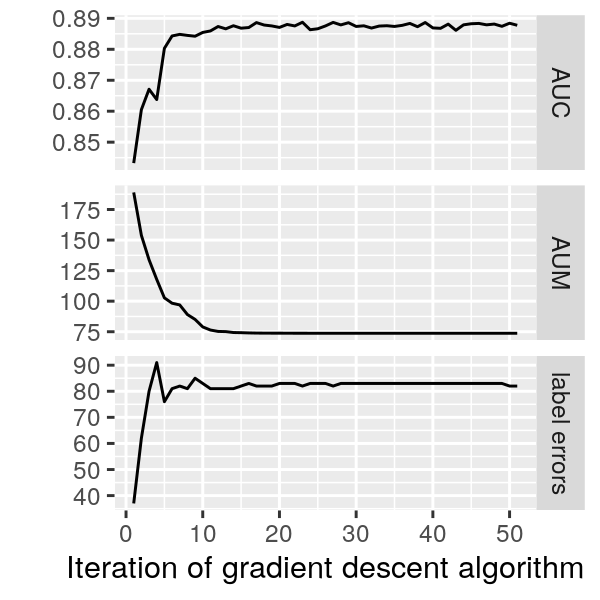
\includegraphics[height=5.5cm]{figure-aum-optimized-iterations.png}
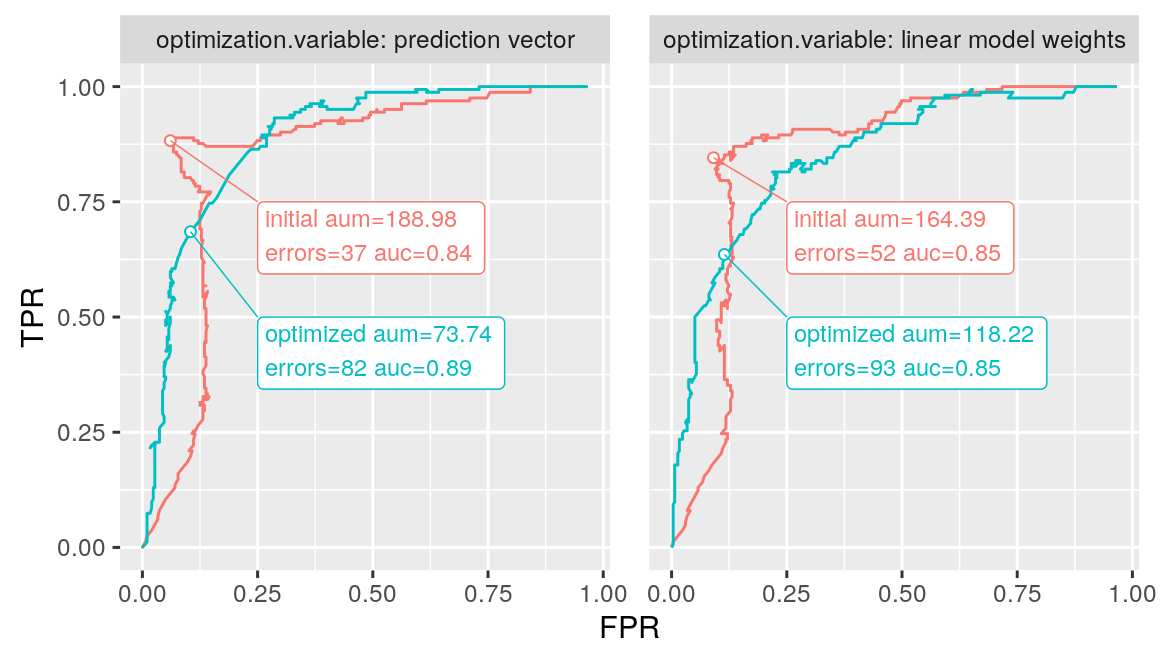
\includegraphics[height=5.5cm]{figure-aum-train-both.png}
\vskip -0.5cm
\caption{
Minimizing the AUM tends to increase AUC and label error rates, with respect to the train set ($n=54$ labeled examples).
\textbf{Left:} we used AUM gradient descent on the $n$-vector of predicted values $\mathbf{\hat y}$ in the train set (initial predictions chosen by minimizing label errors for each example). Decreases in AUM happen during the same iterations as increases in AUC and label error rates. 
\textbf{Middle:} ROC curves before and after using AUM gradient descent on the $n$-vector of predicted values (dot shows the point on each ROC curve with minimum label errors).
\textbf{Right:} optimizing the $p$-vector of weights in a linear model ($p=27$ features, initial weights minimize an un-regularized squared hinge loss). 
Note that AUC=0.85 is unchanged by the optimization but AUM decreases and error rate increases.
}
\label{fig:aum-optimized}
\end{center}
\vskip -0.2in
\end{figure*}


%   pos.or.neg.vec <- c(min=-1, max=1)
%   for(min.or.max in names(pos.or.neg.vec)){
%     pos.or.neg <- pos.or.neg.vec[[min.or.max]]
%     fp.fn.join <- fp.fn.totals[
%       fp.fn.problems,
%       .(fp, fn, min.fp.fn, fp.prb.diff, fn.prb.diff),
%       on=structure("thresh", names=paste0(min.or.max, ".thresh"))]
%     for(fX in c("fp", "fn")){
%       set(
%         fp.fn.join,
%         j=paste0(fX, ".adj"),
%         value=fp.fn.join[[fX]]+
%           pos.or.neg*fp.fn.join[[paste0(fX, ".prb.diff")]]
%       )
%     }
%     fp.fn.join[, min.adj := pmin(fp.adj, fn.adj)]
%     set(
%       fp.fn.problems,
%       j=paste0("deriv.", min.or.max),
%       value=fp.fn.join[, pos.or.neg*(min.adj - min.fp.fn)]
%     )
%   }
%   fp.fn.problems[pred, .(
%         lo=sum(deriv.min, na.rm=TRUE),
%         hi=sum(deriv.max, na.rm=TRUE)
%       ), by=.EACHI, on=problem.vars]

\subsection{Pseudocode and complexity analysis}
We propose to compute the matrix of directional derivatives using Algorithm~\ref{alg:gradient-computation} which inputs a prediction vector $\mathbf {\hat y}\in\mathbb R^n$ and error functions $E_i$.
These error functions are exact representations of the piecewise constant $\text{FP}_i, \text{FN}_i$ functions in terms of intervals.
%Changes in these error functions are used to compute the set $S_i$ of breakpoints for each example $i$.
The time complexity of computing the matrix of directional derivatives 
%via Algorithm~\ref{alg:gradient-computation} 
is the same as computing the AUM itself.
The total number of operations is proportional to the total number of breakpoints in the error functions, $B = \sum_{i=1}^n |S_i(\mathbf{\hat{y}})|$.
Therefore if we assume there are on average $b$ breakpoints in each error function, then the total number of breakpoints is $B=O(bn)$.
The time to compute


\begin{algorithm}[tb]
  \caption{AUM and Gradient Computation}
  \label{alg:gradient-computation}
\begin{algorithmic}[1]
  \STATE {\bfseries Input:} 
  Predictions $\mathbf{\hat y}\in\mathbb R^n$, 
  $j\in\{1,\dots,J\}$ breakpoints in error functions  $p_j,\Delta\text{fp}_j,\Delta\text{fn}_j,I_j$.
  \STATE Initialize to zero the $\text{AUM}\in\mathbb R$ and directional derivatives $\mathbf D\in\mathbb R^{n\times 2}$.
  \STATE  $S_1,\dots,S_n\gets \textsc{SORTEDTOTALS}()$
  \STATE  $T\gets \textsc{TotalsTable}(\mathbf{\hat y}, E_1, \dots, E_n)$
  \FOR{$i\in\{1,\dots,n\}$}
  \STATE $S_i \gets \textsc{ErrorDiffs}(\hat y_i, E_i)$
  \FOR{$d\in\{-1,1\}$}
  \STATE $\mathbf D_{i,d}\gets \textsc{Derivative}(d, S_i, \text{TotalsTable})$
  \ENDFOR
  \ENDFOR
  \STATE {\bfseries Output:} matrix $\mathbf D$ of directional derivatives.
\end{algorithmic}
\end{algorithm}

\begin{algorithm}[tb]
  \caption{SORT SUBROUTINE}
  \label{alg:sort-subroutine}
\begin{algorithmic}[1]
  \STATE {\bfseries Input:} 
  Predictions $\mathbf{\hat y}\in\mathbb R^n$, 
  $j\in\{1,\dots,J\}$ breakpoints in error functions  $p_j,\Delta\text{fp}_j,\Delta\text{fn}_j,I_j$.
  \STATE Initialize to zero the $\text{AUM}\in\mathbb R$ and directional derivatives $\mathbf D\in\mathbb R^{n\times 2}$.
  \STATE  $t_j\gets p_j - \hat y_{I_j} \forall j\in\{1,\dots,$
  \STATE  $S_1,\dots,S_n\gets \textsc{SortedIndices}()$
  \STATE  $T\gets \textsc{TotalsTable}(\mathbf{\hat y}, E_1, \dots, E_n)$
  \FOR{$i\in\{1,\dots,n\}$}
  \STATE $S_i \gets \textsc{ErrorDiffs}(\hat y_i, E_i)$
  \FOR{$d\in\{-1,1\}$}
  \STATE $\mathbf D_{i,d}\gets \textsc{Derivative}(d, S_i, \text{TotalsTable})$
  \ENDFOR
  \ENDFOR
  \STATE {\bfseries Output:} matrix $\mathbf D$ of directional derivatives.
\end{algorithmic}
\end{algorithm}


\subsection{Gradient descent algorithm for predicted values}
\label{sec:gradient-descent}

We propose gradient descent optimization algorithms that use the AUM directional derivatives computed using Theorem~\ref{thm:directional-derivs}.
%and Algorithm~\ref{alg:gradient-computation}.
First to study how minimizing the train AUM affects the train AUC, we propose to optimize the $n$-vector of predictions $\mathbf{\hat{y}}$.
When the AUM is non-convex, the initialization of the algorithm is important. Therefore when optimizing the vector of predictions, we propose initializing each $\hat y_i$ to a value with minimum label errors, 
\begin{equation}
    \hat y_i^{(0)} = \argmin_x 
    \text{FP}_i(x) + 
    \text{FN}_i(x).
\end{equation}
After initialization we need to compute a descent direction; typically the negative gradient is used.
Although the gradient of the AUM is not defined at every point, we have observed that our gradient descent algorithm empirically almost always stays at differentiable points (i.e., columns of directional derivative matrix are equal).
    % ## Some non-differentiable points that were actually observed!
    % ## data=DNA fold=1 loss=aum.rate step=0.001000
    % ##              [,1]         [,2]
    % ## [1,] -0.001956947 -0.001175589
    % ## data=DNA fold=1 loss=aum.rate step=1000.000000
    % ##               [,1] [,2]
    % ## [1,] -0.0006463963    0
However, we have observed a few cases where the gradient descent algorithm visits non-differentiable points, for which there is at least one row in the directional derivative matrix with entries that are not equal. 
Examples of such directional derivative rows $[\nabla_{\mathbf v(-1,i)}\text{AUM}(\mathbf{\hat{y}}),\nabla_{\mathbf v(1,i)}\text{AUM}(\mathbf{\hat{y}})]$ that we have observed include $[-0.0019, -0.0011]$ and $[-0.0006, 0]$, both of which indicate that the loss would increase if the predicted value is decreased. 
The descent direction we propose to use is therefore the negative mean of these two directional derivatives, $-[\nabla_{\mathbf v(-1,i)}\text{AUM}(\mathbf{\hat{y}})+\nabla_{\mathbf v(1,i)}\text{AUM}(\mathbf{\hat{y}})]/2$.
We also perform line search via grid search in order to obtain a step size $\alpha^{(j)}$ which results in the largest decrease in AUM.
Also let $\beta^{(j)}$ be an intercept or threshold with minimal error after taking the line search step (it only affects the label error/accuracy and not the AUM).
Note that this intercept can be efficiently computed at the same time as the AUM and its directional derivative matrix, by a simple linear scan over all thresholds.
We then perform gradient descent updates for each iteration $j\in\{0,1,\dots\}$ via
\begin{equation}
    \mathbf{\hat y}^{(j+1)} = \mathbf{\hat y}^{(j)} - \alpha^{(j)} \mathbf {\bar D}_\text{AUM}(\mathbf {\hat y}^{(j)}) + \beta^{(j)}.
\end{equation}
%TODO we could add equation for \beta^j in terms of argmin_t FPT(y + t) + FNT(y + t)

\begin{figure*}[t]
\vskip 0.2in
\begin{center}
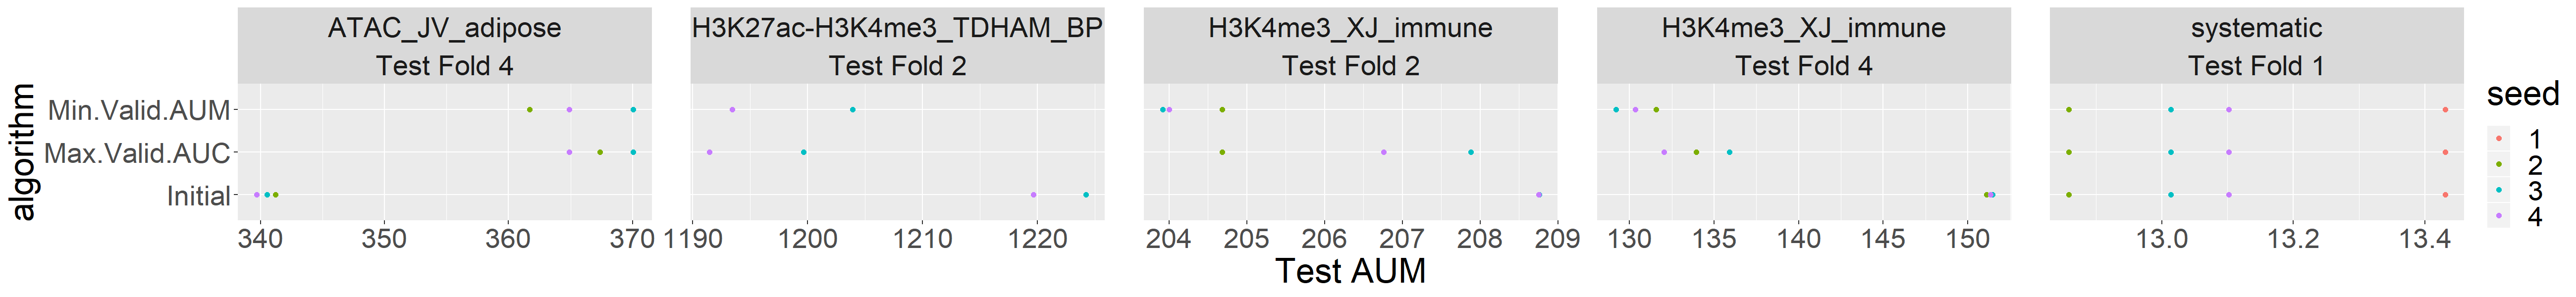
\includegraphics[width=\textwidth]{figure-test-aum-comparison.png}
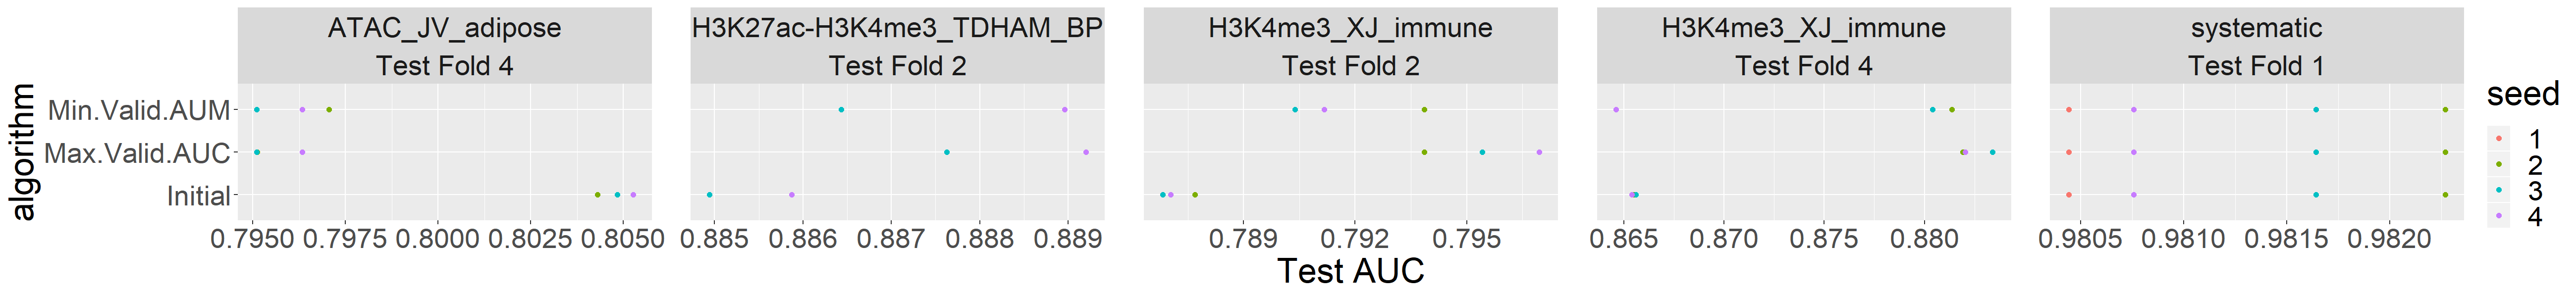
\includegraphics[width=\textwidth]{figure-test-auc-comparison.png}
\vskip -0.5cm
\caption{
Linear model which minimizes AUM via gradient descent results in maximizing AUC on held-out test data.
Algorithm (y axis) shows how number of iterations was chosen, by minimizing validtion AUM, maximizing validation AUC, or taking the initial iteration.
Each of five columns from left to right shows results for four random seeds on a given data set and test fold.
% TODO n=? p=?
% \textbf{Left:}: The left panel shows a model that selected a worse AUM and worse AUC than the initial model. 
% \textbf{Middle}: The middle 3 panels show results for datasets where our K-Fold cross validation algorithm was successful in optimizing the AUM/AUC. 
% \textbf{Right}: The right panel shows a dataset where our initial model was already at a local minimum of the validation AUM/AUC with 4 different random initializations.
}
\label{fig:test-aum-comparison}
\end{center}
\vskip -0.2in
\end{figure*}

\subsection{Gradient descent algorithm for linear model}
\label{sec:linear-model}
In the context of making predictions on a held-out test set, we consider a linear model $f(\mathbf x) = \mathbf w^\intercal \mathbf x + \beta$ parameterized by a weight vector $\mathbf w\in\mathbb R^p$ to optimize via gradient descent, and an intercept $\beta\in\mathbb R$ optimized via a linear scan to find a threshold with minimum label error.
Let $\mathbf X\in\mathbb R^{n\times p}$ be the feature/input matrix, so $\mathbf X \mathbf w+\beta\in\mathbb R^n$ is the vector of predicted values on the train set.
We consider an intialization $\mathbf{w}^{(0)}$ based on minimizing a convex squared hinge loss with L1 regularization \citep{Hocking2013icml}.
This convex loss function has a minimum for each example at predicted values that achieve minimum label errors, so we expect this initialization to have large accuracy but not necessarily large AUC.
Again let $\alpha^{(j)}$ be the line search step size, and let $\beta^{(j)}$ be an intercept with minimal train error.
We perform gradient descent for each iteration $j\in\{0,1,\dots\}$ via
\begin{equation}
    \mathbf{w}^{(j+1)} = \mathbf{w}^{(j)} - \alpha^{(j)}\mathbf X^\intercal \mathbf {\bar D}_\text{AUM}(\mathbf X \mathbf w^{(j)}   + \beta^{(j)}).
\end{equation}
To regularize the model we propose using early stopping (number of  iterations chosen by minimizing AUM or maximizing AUC with respect to a held-out validation set).


\section{Empirical Results}
\label{sec:results}
We empirically study AUM minimization in the context of changepoint detection problems, because they have non-monotonic FP and FN functions.
Our goal is to demonstrate that AUM minimization can result in AUC maximization with respect to train and test data.
\subsection{AUM gradient descent optimizes train AUC}

In this experiment our goal was to demonstrate that minimizing the AUM results in maximizing the AUC in the train set. 
We used the chipseq data (a benchmark for labeled changepoint detection) from the UCI repository \citep{asuncion2007uci}, treating each (set.name, fold) as a different train set, with pre-processing as previously described.\footnote{
\small \href{https://github.com/tdhock/feature-learning-benchmark}{github.com/tdhock/feature-learning-benchmark}}
In brief, for each labeled example, changepoint models were computed for a range of penalty values, which resulted in models with a range of changepoints (some with few changepoints, others with many).
Then the label error rate for each model was computed, along with a penalty $\hat \lambda_i$ which resulted in minimum label errors for each labeled example $i$.
Finally these penalty values were used as the initial prediction vector $\mathbf{\hat y} = [ -\log\hat\lambda_1 \cdots -\log\hat\lambda_n]$, which was used as the optimization variable in an AUM gradient descent algorithm. 
A line search was used for the step size so that the AUM was guaranteed to decrease at each iteration. 
Overall there were 68 different train sets with the number of labeled examples ranging from $n=7$ to 1011.
% > fold.counts[, list(
% +   folds=.N,
% +   min.examples=min(examples),
% +   max.examples=max(examples)
% + )]
%   folds min.examples max.examples
% 1:    68            7         1011

We expected that by using the predicted values directly as the optimization variable in gradient descent, we should be able to obtain ROC curves that were significantly different from the initialization (hopefully with larger AUC, even though the initialization came from minimizing the label error independently for each example).
In a small number of train sets we observed that the optimization resulted in little or no change to both AUM and AUC; this happened when the initialization was close to or at a stationary point of the AUM (for example, when AUM=0 and AUC=1).
However in most of the train sets we observed that minimizing the AUM results in increased AUC (on the train set). 
                    % set.name fold examples labels
% 64:        H3K4me3_XJ_immune    4       54    351
% > test.fold.breaks[, .(
% +   mean.breaks=mean(breaks),
% +   examples=.N
% + )]
%   mean.breaks examples
% 1:    37.07407       54
In one representative train set (H3K4me3\_XJ\_immune fold 4 which has $n=54$ labeled examples with $b=37.1$ breakpoints per average in each error function), we observed that the AUC and label error rate increases during the same iterations that the AUM decreases (Figure~\ref{fig:aum-optimized}, left).
Before optimization the ROC curve was highly non-monotonic with a sharp point in the upper left corner; after AUM optimization the ROC curve became more regular with increased area (Figure~\ref{fig:aum-optimized}, middle).
This result suggests that AUM gradient descent can be used to maximize the AUC, although the label error rate also increases.

We performed a second experiment, this time optimizing  $p=27$ weights in a linear model parameter vector which was used to compute a prediction for each of the $n=54$ labeled examples.
The weights were initialized by using a gradient descent algorithm to minimize an un-regularized squared hinge loss that is a convex relaxation of the label error \citep{Hocking2013icml}.
We expected the constraints of the linear model to reduce the accuracy with respect to the previous experiment (direct optimization of predicted values).
We observed that after optimizing the weights using AUM gradient descent, the train AUC remained the same, but the train error rate increased (Figure~\ref{fig:aum-optimized}, right).
This experiment shows that the constraints of a linear model can prevent AUM minimization from resulting in AUC maximization (even in a data set for which it is possible to achieve larger AUC values).


\begin{figure*}[t]
\vskip 0.2in
\begin{center}
 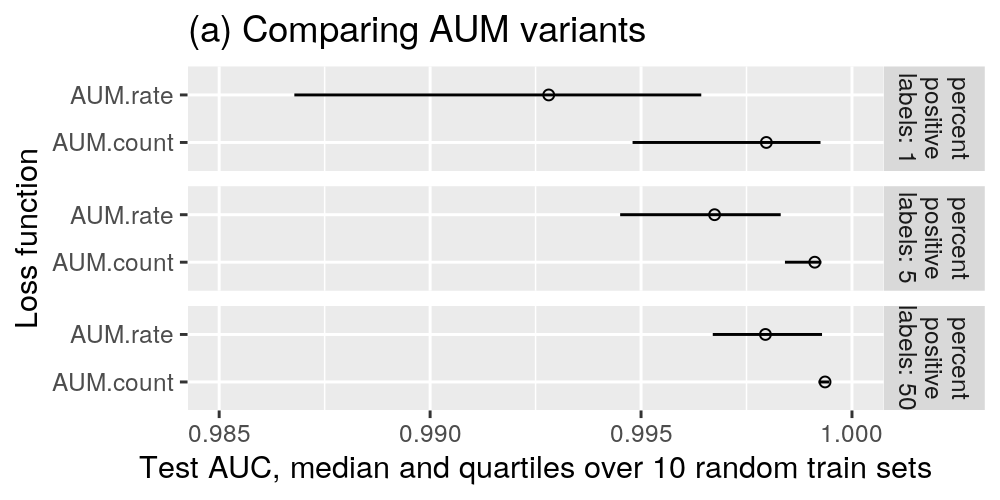
\includegraphics[width=0.49\textwidth]{figure-unbalanced-grad-desc-aum.png}
 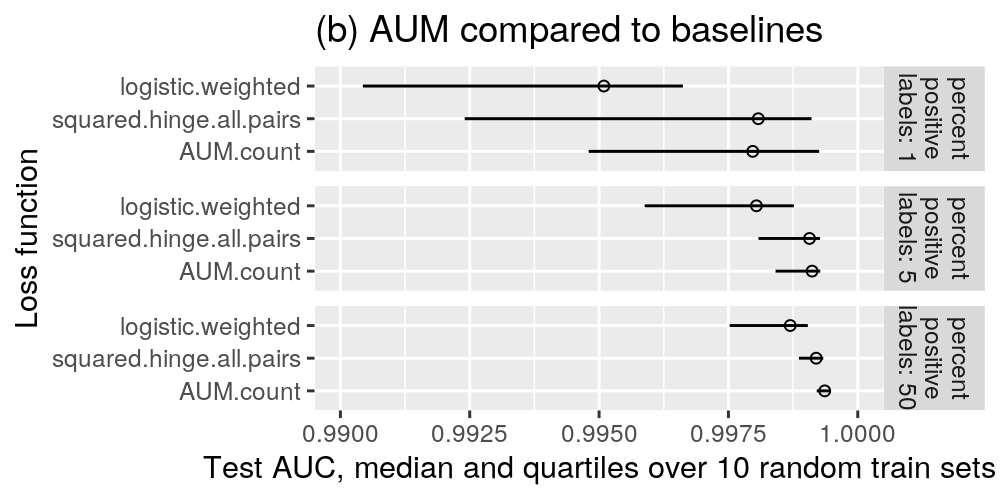
\includegraphics[width=0.49\textwidth]{figure-unbalanced-grad-desc.png}
\vskip -0.5cm
\caption{
Test AUC in binary classification (images of 0/1 digits). Fixed test set with balanced classes (50\% positive, 50\% negative labels), and three train sets with different class imbalance (1\%, 5\%, 50\% positive labels). \textbf{Left (a):} AUM count is more accurate than AUM rate. \textbf{Right (b):} AUM count is at least as accurate as baselines, and sometimes more accurate.}
\label{fig:test-binary}
\end{center}
\vskip -0.2in
\end{figure*}



\subsection{Test AUM and AUC in changepoint problems}

In these experiments, the goal was to demonstrate that test AUC correlates with test AUM using our proposed linear model based on AUM minimization.
We considered supervised changepoint detection data sets from a public repository.\footnote{\small\href{https://github.com/tdhock/neuroblastoma-data}{github.com/tdhock/neuroblastoma-data}} 
It included pre-defined fold IDs that we used to define train/test splits over labeled examples of changepoint detection problems.
In the five train sets that we analyzed (Figure~\ref{fig:test-aum-comparison}), the number of labeled examples ranged from $n=216$ to 3322, the number of features from $p=26$ to 117, and the mean number of breakpoints in each error function from $b=1$ to 6.7.
% > meta.dt[, .(data.name, test.fold, features, n.train, mean.breaks)]
%                   data.name test.fold features n.train mean.breaks
% 1:          ATAC_JV_adipose         4       29     341    6.665689
% 2: H3K27ac-H3K4me3_TDHAM_BP         2       26    1865    4.145845
% 3:        H3K4me3_XJ_immune         2       28     216    5.902778
% 4:        H3K4me3_XJ_immune         4       28     216    6.134259
% 5:               systematic         1      117    3322    1.010235
% > (meta.stats <- meta.tall[, .(
% +   min=min(value),
% +   max=max(value)
% + ), by=variable])
%       variable        min         max
% 1:    features  26.000000  117.000000
% 2:     n.train 216.000000 3322.000000
% 3: mean.breaks   1.010235    6.665689
As explained in Section~\ref{sec:linear-model}, our initialization and baseline was a linear model learned via gradient descent on a convex squared hinge loss with L1 regularization \citep{Hocking2013icml}.
% It should be noted that this algorithm is o random assignment of folds to choose the regularization. includes an internal cross-validation loop to choose the regularization parameter, so it is a randomized algorithm, and the output of it varies with the random seed it is given.
To determine the extent to which the result depends on random initialization, we used four different seeds to select four different initial models. 
Some of the random seeds resulted in the same initial weights, despite having different seeds.

For each train set and random seed we used AUM gradient descent and selected the number of iterations via 4-fold cross-validation (take mean validation AUC/AUM over folds, then select iterations by maximizing AUC or minimizing AUM).
% Our first version of our descent included a test/subtrain/validation split.
% The chosen number of iterations for our model was iteration that had the lowest validation AUM.
% However, after noticing this method resulted in a poor selection of the number of iterations for minimizing the test AUM, we transitioned to using K-Fold cross validation with K = 4 folds, and use the iteration that minimized the mean validation AUM as the selected number of iterations for our model.
% This minimized the test AUM most of the time, but still showed some inconsistencies.
% Since we are indirectly trying to optimize the AUC, we selected the model's number of iterations based off of the maximum mean validation AUC, and compared the test AUM/AUC with the chosen iteration.
%In Figure~\ref{fig:test-aum-comparison}, we compared these two methods (min AUM vs max AUC) to see which one was better for hyper-parameter tuning. 
In general we observed that both methods for selecting the number of iterations resulted in increased test AUC and decreased test AUM (middle three panels of Figure~\ref{fig:test-aum-comparison}). 
However for some data the AUM gradient descent did not improve over the initialization (left and right panels).
This can be explained because some splits had very different train and test sets (left) or 
%monotonic ROC curves which cause initialization at a stationary point of the AUM
the selected number of gradient descent iterations was zero
(right). 
Overall these real data experiments indicate that AUM minimization often results in AUC maximization on held-out test data.




\begin{figure*}[t]
\vskip 0.2in
\begin{center}
TODO binary 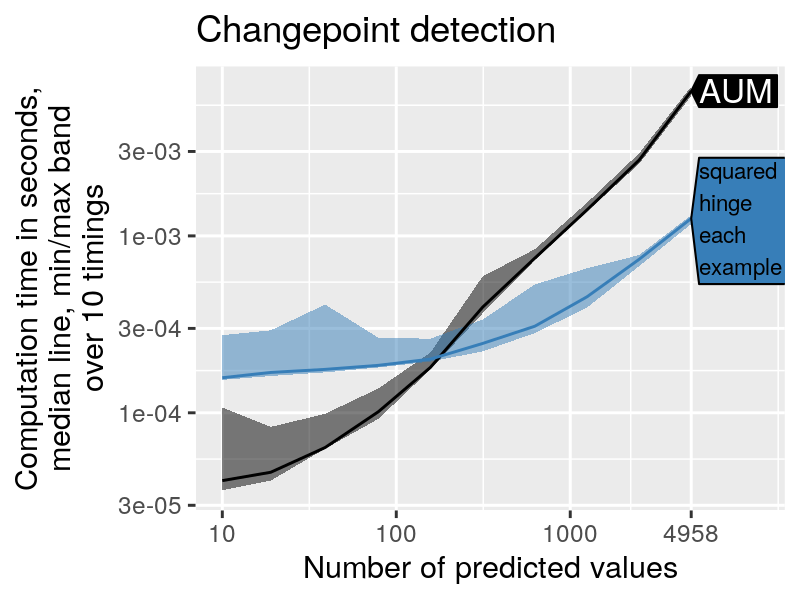
\includegraphics[width=0.4\textwidth]{figure-aum-grad-speed-random.png}
\vskip -0.5cm
\caption{
Speed comparison, time to compute gradient of various loss functions. \textbf{Left:} binary classification TODO. \textbf{Right:} for changepoint detection problems we compared AUM (log-linear) to a squared hinge loss (linear) summed over each of the $N$ labeled examples in the changepoint data set.
}
\label{fig:test-speed}
\end{center}
\vskip -0.2in
\end{figure*}

\subsection{Test AUC in binary classification}

The goal in this section was to demonstrate study the accuracy of our proposed AUM loss function in unbalanced binary classification problems.
Our experiment used the zip.train and zip.test image classification data\footnote{\url{https://web.stanford.edu/~hastie/ElemStatLearn/}} from \citep{Hastie2009}.
Each input is a $16\times 16$ image which is represented by a vector $x\in\mathbb [-1,1]^{256}$.
There are 10 classes (one for each digit), but we only used two classes (0/1) in order to study binary classification.
For both the \texttt{zip.train} and \texttt{zip.test} files, we discarded some $y_i=0$ labels in order to obtain sets with equal numbers of positive and negative labels (total 2010 in train, 528 in test).
Then we generated 10 different train sets by randomly selecting 1000 observations with a class balance in $\{1\%, 5\%, 50\%\}$.
The goal is to learn from the unbalanced train set data and then provide accurate predictions (as measured by AUC) on the balanced test set.

We compared several different algorithms TODO.
In this work we defined the AUM as the area under the minimum of false positive and false negative \emph{counts}, but we could instead use \emph{rates} which would correspond to assigning equal weights to the two classes of errors.



\subsection{Speed comparison}

The goal of this section is to show that AUM gradient computation has comparable speed to existing loss functions. 
TODO binary Jon.
We also did a speed test in the context of real changepoint detection problems, by comparing the AUM to a squared hinge loss summed over each of the $N$ labeled examples \citep{Hocking2013icml}. 
We observed that the AUM gradient is slower than the squared hinge loss complexity (Figure~\ref{fig:test-speed}, right).
For example we observed about 10ms for AUM versus 1ms for the squared hinge for about 5000 examples with approximately 5 changes in error function per example.
Overall these data show that the AUM has comparable speed to previously proposed loss functions for AUC  optimization in binary classification, and changepoint detection.




%TODO Binary classification?


\section{Discussion and conclusions}
\label{sec:discussion}

In this paper we proposed the new AUM loss function which can be used in the context of prediction problems with false positive/negative rates such as in supervised binary classification and changepoint detection.
We proposed a new algorithm for efficiently computing the AUM and its directional derivatives, then showed how the AUM can be directly optimized in a linear gradient descent learning algorithm. 

% TODO compare with previous algorithms which attempt AUC opt.

We have shown that in changepoint detection problems with non-monotonic FP/FN functions, there is a tradeoff between AUC and accuracy that does not exist in binary classification problems.
If maximizing accuracy with respect to the labels is important, we can use existing convex loss functions which are surrogates to minimizing label error rates \citep{Hocking2013icml}.
If maximizing AUC is important, then we can minimize our new AUM loss function which we have shown empirically results in AUC maximization (but lower accuracy).
This tradeoff between AUC and accuracy means that the max accuracy model results in a highly non-monotonic ROC curve with many sub-optimal points, whereas the max AUC model has a more regular ROC curve (Figure~\ref{fig:aum-optimized}).

% or variant which ignores the amount of threshold and instead counts number of thresholds (like ROC only depends on number of thresholds, not the amount) this would amount to removing the        $\tau(\mathbf {\hat y})_{q} - \tau(\mathbf {\hat y})_{q-1}$ term in (\ref{eq:AUM-computation}) -> would not work, piecewise constant so not differentiable, can't use gradient descent.

For future work, we would like to consider several variants of our new AUM loss function.
In this work we proposed a full gradient algorithm (takes a step defined by all training examples), and we would additionally like to explore a batch variant (takes a step defined by a subset of training examples), which is non-trivial since the AUM is not separable over training examples.
Finally our current algorithm uses a grid search over step sizes, but a faster learning algorithm could potentially be obtained by exploiting the piecewise linear nature of the AUM during the step size computation.
%area under something else (maybe remove all ROC points which are sub-optimal to some other point in either FPR or TPR).

\paragraph{Author contributions.} TODO. 

\paragraph{Reproducible Research Statement.} All of the software and data required to make the figures in this paper can be downloaded from \url{https://github.com/tdhock/max-generalized-auc}. 
%An R package which implements the AUM gradient computation is available at URL HIDDEN DURING PEER REVIEW.

% Acknowledgements should only appear in the accepted version.
% \section*{Acknowledgements}

% \textbf{Do not} include acknowledgements in the initial version of
% the paper submitted for blind review.

% If a paper is accepted, the final camera-ready version can (and
% probably should) include acknowledgements. In this case, please
% place such acknowledgements in an unnumbered section at the
% end of the paper. Typically, this will include thanks to reviewers
% who gave useful comments, to colleagues who contributed to the ideas,
% and to funding agencies and corporate sponsors that provided financial
% support.


\bibliography{refs}
\bibliographystyle{icml2021}

\end{document}
